\documentclass[../main.tex]{subfiles}
\begin{document}
\chapter{Esperimenti e risultati}

In questo capitolo vengono presentati gli esperimenti effettuati e le prestazioni ottenuti dallo script di conversione, successivamente i test fatti con Stratosphere IPS sulla creazione di modelli comportamentali per verificare l'accuratezza della conversione dei flows.

\section{Software utilizzati}

Per lo sviluppo del programma per la conversione dei file e per l'utilizzo di Stratosphere IPS è stata creata una piattaforma dedicata alla Security Analytics tramite l'utilizzo di \textit{VirtualBox} con una installazione del sistema operativo Ubuntu 16.04 LTS.


\begin{verse}
				\textbf{VirtualBox} è un software gratuito e open source per l'esecuzione di macchine virtuali che supporta Windows, GNU/Linux e macOS come sistemi operativi host ed è in grado di eseguire Windows, GNU/Linux, OS/2 Warp, BSD come ad esempio OpenBSD, FreeBSD e infine Solaris e OpenSolaris come sistemi operativi guest \cite{virtualbox}. 
\end{verse}

Per controllare se la conversione viene effettuata correttamente si è usato il software Stratosphere IPS per creare e utilizzare dei modelli impiegati per fare \textit{anomaly detection} su del traffico di rete. I flows sono stati convertiti nel formato compatibile da Argus ad nProbe e infine di nuovo ad Argus per controllare che non ci siano delle perdite di informazioni vitali che alterino il funzionamento dell'IDPS.

La figura seguente descrive il processo di conversione. Ad ogni conversione effettuata è prevista una perdita di informazioni dovuta al tipo di campi utilizzati nei diversi formati e alla loro formattazione.

\begin{figure}[H]
				\centering
				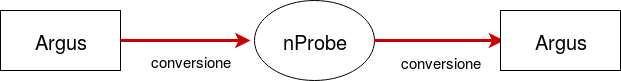
\includegraphics[scale=0.5]{conversion.png}
				\caption{Processo di conversione}
\end{figure}

\section{Installazione Stratosphere IPS}
Sulla macchina virtuale è stato installato il framework di Stratospehere IPS. Di seguito i passaggi effettuati per l'installazione \cite{stf}.

\begin{itemize}
				\item Installazione del programma git 2.7.4
\begin{lstlisting}[language=bash]
$ sudo apt install git
\end{lstlisting}

				\item Clonazione repository github del framework
\begin{lstlisting}[language=bash]
$ git clone https://github.com/stratosphereips/StratosphereTestingFramework
\end{lstlisting}

				\item Installazione del programma python-pip
\begin{lstlisting}[language=bash]
$ sudo apt install python-pip
\end{lstlisting}
\end{itemize}
				
\begin{itemize}
				\paragraph{Installazione dipendenze per Stratosphere IPS}

				\item prettytable 0.7.2-3
\begin{lstlisting}[language=bash]
$ sudo apt install python-prettytable
\end{lstlisting}

				\item transaction 1.4.3-3
\begin{lstlisting}[language=bash]
$ sudo apt install python-transaction
\end{lstlisting}

				\item persistent 4.1.1-1build2
\begin{lstlisting}[language=bash]
$ sudo apt install python-persistent
\end{lstlisting}

				\item zodb 5.4.0
\begin{lstlisting}[language=bash]
$ sudo pip install zodb
\end{lstlisting}

				\item sparse 1.1-1.3build1
\begin{lstlisting}[language=bash]
$ sudo apt install python-sparse
\end{lstlisting}

				\item dateutil 2.4.2-1
\begin{lstlisting}[language=bash]
$ sudo apt install python-dateutil
\end{lstlisting}


\end{itemize}

\section{Installazione di Argus}

Per generare i netflow dal traffico di rete è necessario avere una istanza di Argus sul computer. I seguenti passaggi sono necessari per la corretta installazione di Argus \cite{stf}.

\begin{itemize}
				\item libpcap 1.7.4-2
\begin{lstlisting}[language=bash]
$ sudo apt install libpcab-dev
\end{lstlisting}

\item bison 3.0.4
\begin{lstlisting}[language=bash]
$ sudo apt install bison
\end{lstlisting}

\item flex 2.6.0-11
\begin{lstlisting}[language=bash]
$ sudo apt install flex
\end{lstlisting}

\item Installazione dell'ultima versione di argus 3.0.8.2 dal sito http://qosient.com/argus/dev/argus-latest.tar.gz

\item Installazione dell'ultima versione di argus-client 3.0.8.2 dal sito http://qosient.com/argus/dev/argus-clients-latest.tar.gz

\end{itemize}
\section{Utilizzo del programma stf\\}
*!*!*!*!*!*!*!*!* Questa parte mi sembra brutta, per ogni riga dovrei caricare un'immagine presa da github, la caption è direttamente la riga sopra !*!*!*!*!*!*!*\newline

Per eseguire il programma lo si esegue con
\begin{lstlisting}[language=bash]
	./stf.py
\end{lstlisting}
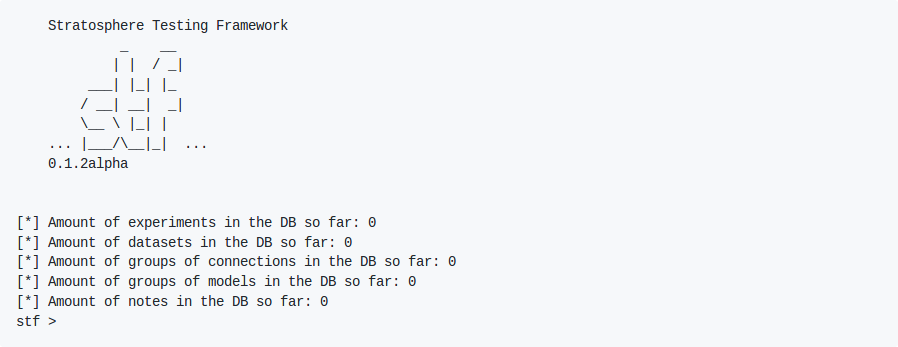
\includegraphics[scale=0.5]{homestf.png}

Per caricare un dataset si utilizza il comando
\begin{lstlisting}[language=bash]
	datasets -c /absolute/path/file.binetflow	
\end{lstlisting}

Per generare la connessione si utilizza il comando
\begin{lstlisting}[language=bash]
	connections -g	
\end{lstlisting}

Infine, per generare i modelli, il comando
\begin{lstlisting}[language=bash]
	models -g	
\end{lstlisting}

Per visualizzare il behavioral model si utilizza il comando
\begin{lstlisting}[language=bash]
	models -L [id]	
\end{lstlisting}
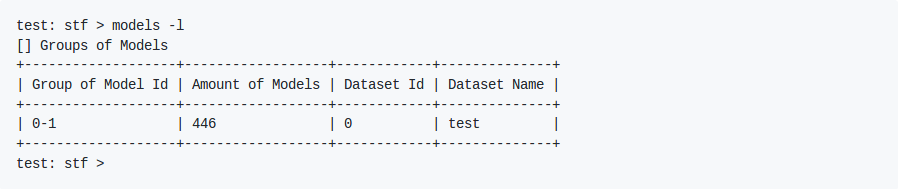
\includegraphics[scale=0.5]{stfmodels.png}
\end{document}

\section{Prestazioni}

Come visto nel capitolo 4, il programma di conversione proposto è efficiente. In questa sezione vengono effettuati dei \textit{benchmark} per analizzare quanto è efficiente e studiare la scalabilità di una soluzione che prevede l'utilizzo di più CPU in parallelo.

\subsection{Benchmark}

Per misurare la velocità del programma si è usato come dataset un intero mese di flows. La dimensione del dataset è di 4,4 Gb per un totale di 43200 file. Le misure sono state realizzate con il programma /usr/bin/time.

Il primo benchmark è stato effettuato su una versione del programma in single core, ovvero che sfrutta la potenza di una sola CPU. I risultati vengono riportati a seguire.

Come si è visto nel capitolo 4, utilizzare una sola CPU oltre a essere estremamente inefficiente, crea anche un file unico in cui vengono salvati tutti i file. La dimensione di questo file è !*!*!
È possibile risolvere il problema della grandezza del file utilizzando un approccio 1:1, cioè di creare un file in output per ogni file in input, ma siccome stiamo utilizzando una sola CPU questo approccia allunga significativamente i tempi di conversione in quanto per ogni file deve essere chiamata una funzione di sistema per la scrittura su file che è la più pesante. Scrivendo solo su un file la chiamata di sistema viene invocata solamente una volta.
\begin{enumerate}
				\item 2:28:03 98\%CPU
				\item 2:27:98 98\%CPU
				\item 2:28:86 98\%CPU
				\item 2:28:97 95\%CPU
				\item 2:24:52 99\%CPU
				\item 2:34:21 94\%CPU
				\item 2:28:36 98\%CPU
				\item 2:35:02 93\%CPU
				\item 2:25:59 99\%CPU
				\item 2:28:75 96\%CPU
\end{enumerate}

La media calcolata è quindi di \textbf{2:28:38 97\%CPU}


\subsection{Benchmark multi core}

Sono stati effettuati 10 test in entrambe le modalità. I risultati vengono riportati a seguire.
Tutti i benchmark sono stati effettuati con \textit{/usr/bin/time}

\begin{enumerate}
				\item 0:54:82 265\%CPU
				\item 0:36:13 375\%CPU
				\item 0:38:24 367\%CPU
				\item 0:40:25 377\%CPU
				\item 0:40:14 368\%CPU
				\item 0:44:28 351\%CPU
				\item 0:41:67 368\%CPU
				\item 0:40:72 383\%CPU
				\item 0:40:83 381\%CPU
				\item 0:41:19 382\%CPU
\end{enumerate}
La media calcolata è quindi di \textbf{0:41:83 362\%CPU}

\begin{figure}[H]
				\centering
				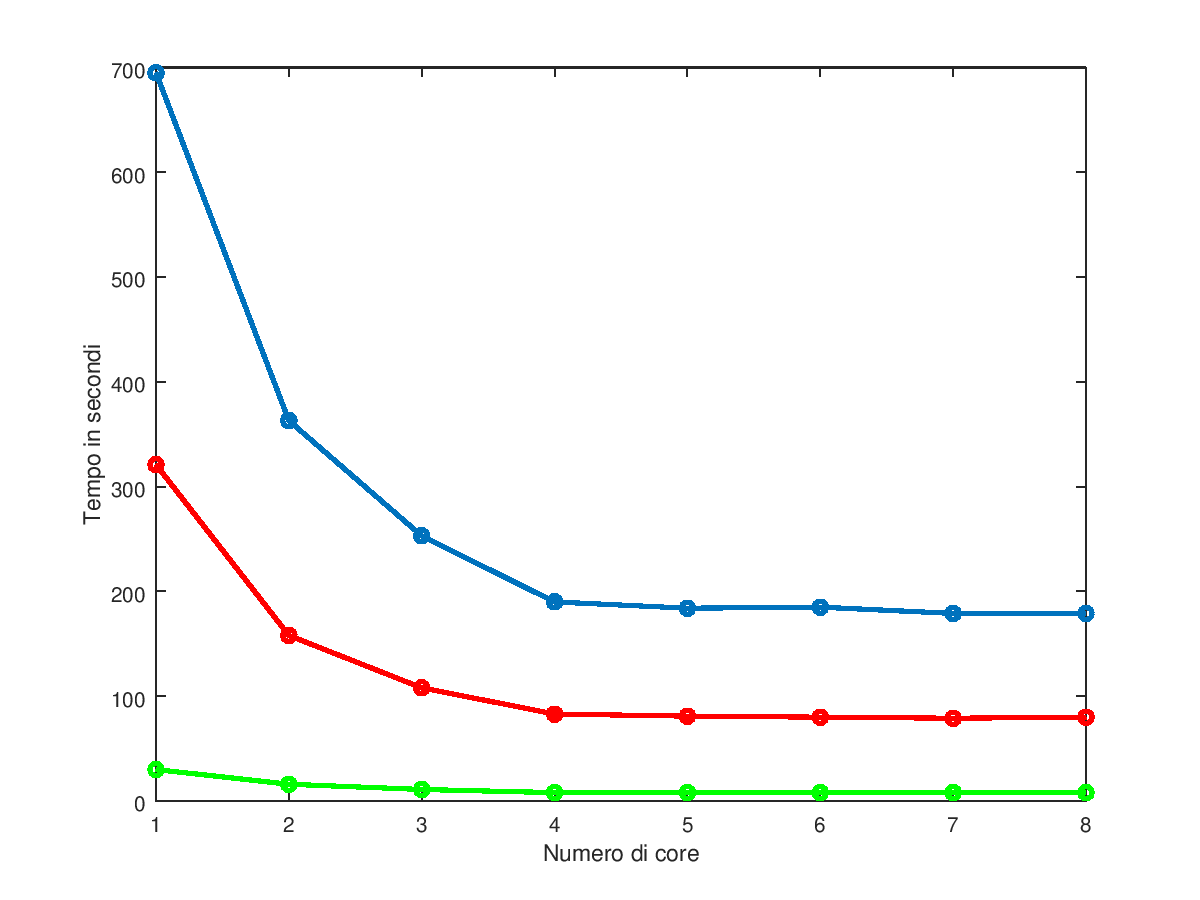
\includegraphics[scale=0.3]{graph1.png}
				\caption{prestazioni}
\end{figure}

\end{document}
